\documentclass[a4paper]{book}
\usepackage{makeidx}
\usepackage{natbib}
\usepackage{graphicx}
\usepackage{multicol}
\usepackage{float}
\usepackage{listings}
\usepackage{color}
\usepackage{ifthen}
\usepackage[table]{xcolor}
\usepackage{textcomp}
\usepackage{alltt}
\usepackage{ifpdf}
\ifpdf
\usepackage[pdftex,
            pagebackref=true,
            colorlinks=true,
            linkcolor=blue,
            unicode
           ]{hyperref}
\else
\usepackage[ps2pdf,
            pagebackref=true,
            colorlinks=true,
            linkcolor=blue,
            unicode
           ]{hyperref}
\usepackage{pspicture}
\fi
\usepackage[utf8]{inputenc}
\usepackage{polski}
\usepackage[T1]{fontenc}

\usepackage{mathptmx}
\usepackage[scaled=.90]{helvet}
\usepackage{courier}
\usepackage{sectsty}
\usepackage[titles]{tocloft}
\usepackage{doxygen}
\lstset{language=C++,inputencoding=utf8,basicstyle=\footnotesize,breaklines=true,breakatwhitespace=true,tabsize=8,numbers=left }
\makeindex
\setcounter{tocdepth}{3}
\renewcommand{\footrulewidth}{0.4pt}
\renewcommand{\familydefault}{\sfdefault}
\hfuzz=15pt
\setlength{\emergencystretch}{15pt}
\hbadness=750
\tolerance=750
\begin{document}
\hypersetup{pageanchor=false,citecolor=blue}
\begin{titlepage}
\vspace*{7cm}
\begin{center}
{\Large \-Calka }\\
\vspace*{1cm}
{\large \-Wygenerowano przez Doxygen 1.7.6.1}\\
\vspace*{0.5cm}
{\small Tue Jun 3 2014 17:27:10}\\
\end{center}
\end{titlepage}
\clearemptydoublepage
\pagenumbering{roman}
\tableofcontents
\clearemptydoublepage
\pagenumbering{arabic}
\hypersetup{pageanchor=true,citecolor=blue}
\chapter{\-Struktura katalogów}
\section{\-Katalogi}
\-Ta struktura katalogów jest posortowana jest z grubsza, choć nie całkowicie, alfabetycznie\-:\begin{DoxyCompactList}
\item \contentsline{section}{prj}{\pageref{dir_9f92f53661fd78c561fa1672d6c740cd}}{}
\end{DoxyCompactList}

\chapter{\-Indeks klas}
\section{\-Lista klas}
\-Tutaj znajdują się klasy, struktury, unie i interfejsy wraz z ich krótkimi opisami\-:\begin{DoxyCompactList}
\item\contentsline{section}{\hyperlink{class_drzewo}{\-Drzewo$<$ K, W $>$} \\*\-Modeluje pojecie drzewa binarnego. \-Jego atrybutem jest klasa \hyperlink{class_wezel}{\-Wezel} }{\pageref{class_drzewo}}{}
\item\contentsline{section}{\hyperlink{class_para}{\-Para$<$ K, W $>$} \\*\-Modeluje pojecie pary. \-Jej atrybutem sa pola zawierajace klucz i wartosci }{\pageref{class_para}}{}
\item\contentsline{section}{\hyperlink{class_tablica}{\-Tablica$<$ K, W $>$} \\*\-Modeluje pojecie tablicy z haszowaniem. \-Klasa modeluje pojecie tablicy z haszowaniem. \-Jej atrybutami sa pola\-: klucz i wartosc }{\pageref{class_tablica}}{}
\item\contentsline{section}{\hyperlink{class_wezel}{\-Wezel$<$ K, W $>$} \\*\-Modeluje pojecie wezla. \-Jego atrybutem jest klasa \hyperlink{class_para}{\-Para} }{\pageref{class_wezel}}{}
\end{DoxyCompactList}

\chapter{\-Indeks plików}
\section{\-Lista plików}
\-Tutaj znajduje się lista wszystkich plików z ich krótkimi opisami\-:\begin{DoxyCompactList}
\item\contentsline{section}{\hyperlink{main_8cpp}{main.\-cpp} \\*\-Plik zawiera glowna funkcje programu }{\pageref{main_8cpp}}{}
\item\contentsline{section}{\hyperlink{simplex_8cpp}{simplex.\-cpp} \\*\-Definicje poszczegolnych funkcji dla klasy \hyperlink{class_simplex}{\-Simplex} }{\pageref{simplex_8cpp}}{}
\item\contentsline{section}{\hyperlink{simplex_8h}{simplex.\-h} \\*\-Plik naglowkowy klasy \hyperlink{class_simplex}{\-Simplex} }{\pageref{simplex_8h}}{}
\end{DoxyCompactList}

\chapter{\-Dokumentacja katalogów}
\hypertarget{dir_0215b0778b526eac775effa7830a5ddd}{\section{\-Dokumentacja katalogu /home/martyna/\-Pulpit/calka/prj/}
\label{dir_0215b0778b526eac775effa7830a5ddd}\index{\-Dokumentacja katalogu /home/martyna/\-Pulpit/calka/prj/@{\-Dokumentacja katalogu /home/martyna/\-Pulpit/calka/prj/}}
}
\-Directory dependency graph for /home/martyna/\-Pulpit/calka/prj/\-:
\nopagebreak
\begin{figure}[H]
\begin{center}
\leavevmode
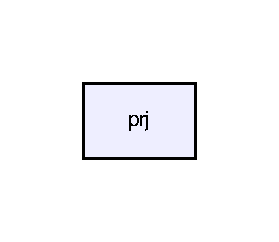
\includegraphics[width=134pt]{dir_0215b0778b526eac775effa7830a5ddd_dep}
\end{center}
\end{figure}
\subsection*{\-Pliki}
\begin{DoxyCompactItemize}
\item 
plik \hyperlink{integral_8cpp}{integral.\-cpp}
\item 
plik \hyperlink{integral_8h}{integral.\-h}
\begin{DoxyCompactList}\small\item\em \-Plik naglowkowy klasy \hyperlink{class_integral}{\-Integral}. \end{DoxyCompactList}\item 
plik \hyperlink{main_8cpp}{main.\-cpp}
\begin{DoxyCompactList}\small\item\em \-Plik zawiera glowna funkcje programu. \end{DoxyCompactList}\end{DoxyCompactItemize}

\chapter{\-Dokumentacja klas}
\hypertarget{class_integral}{\section{\-Dokumentacja klasy \-Integral}
\label{class_integral}\index{\-Integral@{\-Integral}}
}


\-Deklaracja klasy \hyperlink{class_integral}{\-Integral}.  




{\ttfamily \#include $<$integral.\-h$>$}

\subsection*{\-Metody publiczne}
\begin{DoxyCompactItemize}
\item 
\hyperlink{class_integral_a3ba4abca152f119d4b95ad7e4dd7f43f}{\-Integral} (double($\ast$\hyperlink{class_integral_a12d960433639c75917e0d0758498b0da}{f})(double))
\item 
double \hyperlink{class_integral_a48e95c56d7710386a6cc7d4c43b618cd}{\-Definite\-Integral} (double from, double to)
\item 
double \hyperlink{class_integral_ac91a8edc240a85b9efcfe3f3b75e585e}{\-Indefinite\-Integral} (double from, double to)
\end{DoxyCompactItemize}
\subsection*{\-Atrybuty prywatne}
\begin{DoxyCompactItemize}
\item 
double($\ast$ \hyperlink{class_integral_a12d960433639c75917e0d0758498b0da}{f} )(double)
\end{DoxyCompactItemize}


\subsection{\-Opis szczegółowy}
\-Deklaracja klasy \hyperlink{class_integral}{\-Integral}. 

\-Definicja w linii 17 pliku integral.\-h.



\subsection{\-Dokumentacja konstruktora i destruktora}
\hypertarget{class_integral_a3ba4abca152f119d4b95ad7e4dd7f43f}{\index{\-Integral@{\-Integral}!\-Integral@{\-Integral}}
\index{\-Integral@{\-Integral}!Integral@{\-Integral}}
\subsubsection[{\-Integral}]{\setlength{\rightskip}{0pt plus 5cm}{\bf \-Integral\-::\-Integral} (
\begin{DoxyParamCaption}
\item[{double($\ast$)(double)}]{f}
\end{DoxyParamCaption}
)}}\label{class_integral_a3ba4abca152f119d4b95ad7e4dd7f43f}


\-Definicja w linii 4 pliku integral.\-cpp.



\subsection{\-Dokumentacja funkcji składowych}
\hypertarget{class_integral_a48e95c56d7710386a6cc7d4c43b618cd}{\index{\-Integral@{\-Integral}!\-Definite\-Integral@{\-Definite\-Integral}}
\index{\-Definite\-Integral@{\-Definite\-Integral}!Integral@{\-Integral}}
\subsubsection[{\-Definite\-Integral}]{\setlength{\rightskip}{0pt plus 5cm}double {\bf \-Integral\-::\-Definite\-Integral} (
\begin{DoxyParamCaption}
\item[{double}]{from, }
\item[{double}]{to}
\end{DoxyParamCaption}
)}}\label{class_integral_a48e95c56d7710386a6cc7d4c43b618cd}


\-Definicja w linii 10 pliku integral.\-cpp.



\-Oto graf wywoływań tej funkcji\-:\nopagebreak
\begin{figure}[H]
\begin{center}
\leavevmode
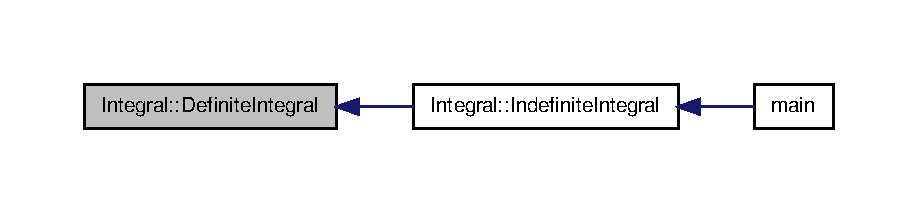
\includegraphics[width=350pt]{class_integral_a48e95c56d7710386a6cc7d4c43b618cd_icgraph}
\end{center}
\end{figure}


\hypertarget{class_integral_ac91a8edc240a85b9efcfe3f3b75e585e}{\index{\-Integral@{\-Integral}!\-Indefinite\-Integral@{\-Indefinite\-Integral}}
\index{\-Indefinite\-Integral@{\-Indefinite\-Integral}!Integral@{\-Integral}}
\subsubsection[{\-Indefinite\-Integral}]{\setlength{\rightskip}{0pt plus 5cm}double {\bf \-Integral\-::\-Indefinite\-Integral} (
\begin{DoxyParamCaption}
\item[{double}]{from, }
\item[{double}]{to}
\end{DoxyParamCaption}
)}}\label{class_integral_ac91a8edc240a85b9efcfe3f3b75e585e}


\-Definicja w linii 29 pliku integral.\-cpp.



\-Oto graf wywołań dla tej funkcji\-:\nopagebreak
\begin{figure}[H]
\begin{center}
\leavevmode
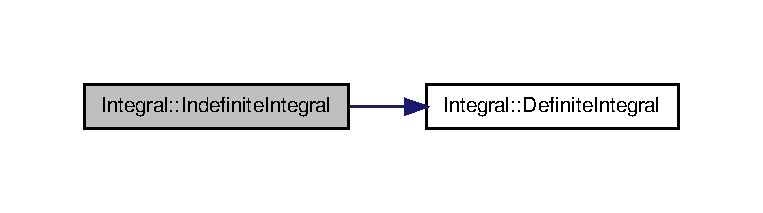
\includegraphics[width=350pt]{class_integral_ac91a8edc240a85b9efcfe3f3b75e585e_cgraph}
\end{center}
\end{figure}




\-Oto graf wywoływań tej funkcji\-:\nopagebreak
\begin{figure}[H]
\begin{center}
\leavevmode
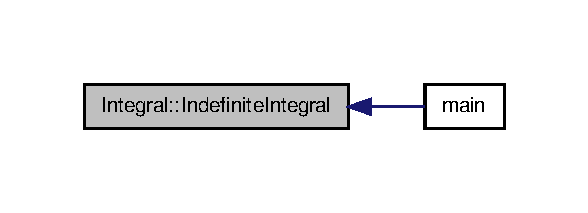
\includegraphics[width=282pt]{class_integral_ac91a8edc240a85b9efcfe3f3b75e585e_icgraph}
\end{center}
\end{figure}




\subsection{\-Dokumentacja atrybutów składowych}
\hypertarget{class_integral_a12d960433639c75917e0d0758498b0da}{\index{\-Integral@{\-Integral}!f@{f}}
\index{f@{f}!Integral@{\-Integral}}
\subsubsection[{f}]{\setlength{\rightskip}{0pt plus 5cm}double($\ast$ {\bf \-Integral\-::f})(double)\hspace{0.3cm}{\ttfamily  \mbox{[}private\mbox{]}}}}\label{class_integral_a12d960433639c75917e0d0758498b0da}


\-Definicja w linii 19 pliku integral.\-h.



\-Dokumentacja dla tej klasy została wygenerowana z plików\-:\begin{DoxyCompactItemize}
\item 
/home/martyna/\-Pulpit/calka/prj/\hyperlink{integral_8h}{integral.\-h}\item 
/home/martyna/\-Pulpit/calka/prj/\hyperlink{integral_8cpp}{integral.\-cpp}\end{DoxyCompactItemize}

\chapter{\-Dokumentacja plików}
\hypertarget{integral_8cpp}{\section{\-Dokumentacja pliku /home/martyna/\-Pulpit/calka/prj/integral.cpp}
\label{integral_8cpp}\index{/home/martyna/\-Pulpit/calka/prj/integral.\-cpp@{/home/martyna/\-Pulpit/calka/prj/integral.\-cpp}}
}
{\ttfamily \#include \char`\"{}integral.\-h\char`\"{}}\*
\-Wykres zależności załączania dla integral.\-cpp\-:\nopagebreak
\begin{figure}[H]
\begin{center}
\leavevmode
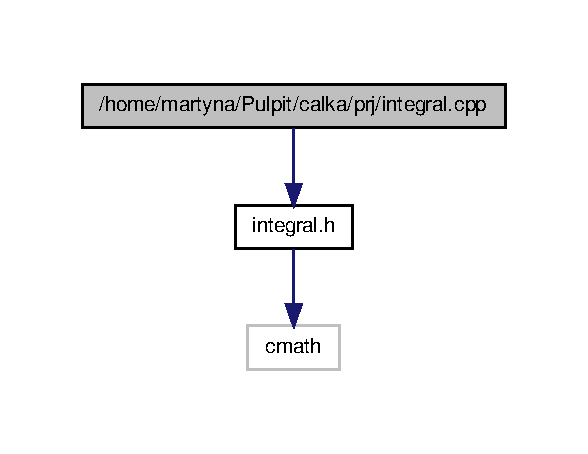
\includegraphics[width=282pt]{integral_8cpp__incl}
\end{center}
\end{figure}

\hypertarget{integral_8h}{\section{\-Dokumentacja pliku /home/martyna/\-Pulpit/calka/prj/integral.h}
\label{integral_8h}\index{/home/martyna/\-Pulpit/calka/prj/integral.\-h@{/home/martyna/\-Pulpit/calka/prj/integral.\-h}}
}


\-Plik naglowkowy klasy \hyperlink{class_integral}{\-Integral}.  


{\ttfamily \#include $<$cmath$>$}\*
\-Wykres zależności załączania dla integral.\-h\-:\nopagebreak
\begin{figure}[H]
\begin{center}
\leavevmode
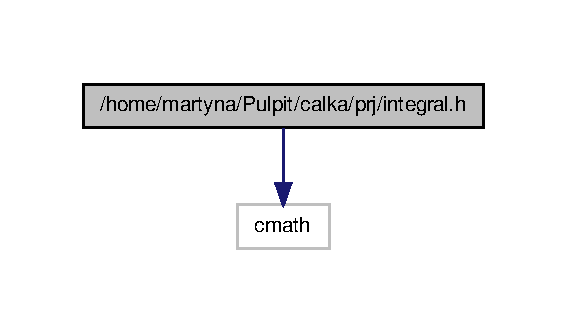
\includegraphics[width=272pt]{integral_8h__incl}
\end{center}
\end{figure}
\-Ten wykres pokazuje, które pliki bezpośrednio lub pośrednio załączają ten plik\-:\nopagebreak
\begin{figure}[H]
\begin{center}
\leavevmode
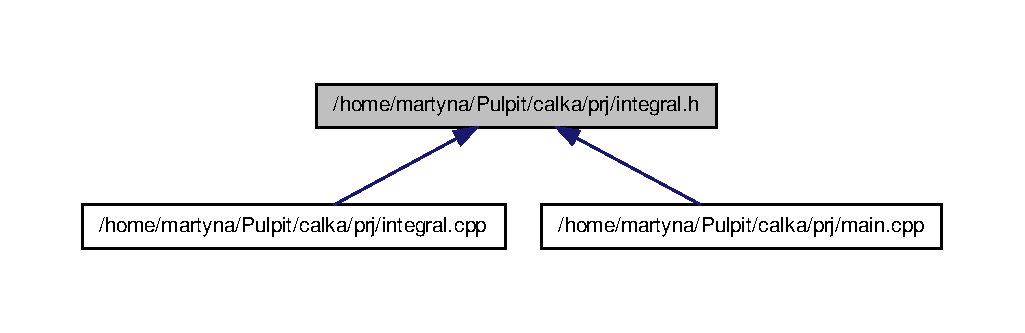
\includegraphics[width=350pt]{integral_8h__dep__incl}
\end{center}
\end{figure}
\subsection*{\-Komponenty}
\begin{DoxyCompactItemize}
\item 
class \hyperlink{class_integral}{\-Integral}
\begin{DoxyCompactList}\small\item\em \-Deklaracja klasy \hyperlink{class_integral}{\-Integral}. \end{DoxyCompactList}\end{DoxyCompactItemize}
\subsection*{\-Zmienne}
\begin{DoxyCompactItemize}
\item 
const int \hyperlink{integral_8h_ad13f184aae302a8bff8bb3dc3c176a24}{\-P\-A\-R\-T\-S\-\_\-\-I\-N\-T\-E\-G\-R\-A\-L} = 1000
\end{DoxyCompactItemize}


\subsection{\-Opis szczegółowy}
\-Plik naglowkowy klasy \hyperlink{class_integral}{\-Integral}. 

\-Definicja w pliku \hyperlink{integral_8h_source}{integral.\-h}.



\subsection{\-Dokumentacja zmiennych}
\hypertarget{integral_8h_ad13f184aae302a8bff8bb3dc3c176a24}{\index{integral.\-h@{integral.\-h}!\-P\-A\-R\-T\-S\-\_\-\-I\-N\-T\-E\-G\-R\-A\-L@{\-P\-A\-R\-T\-S\-\_\-\-I\-N\-T\-E\-G\-R\-A\-L}}
\index{\-P\-A\-R\-T\-S\-\_\-\-I\-N\-T\-E\-G\-R\-A\-L@{\-P\-A\-R\-T\-S\-\_\-\-I\-N\-T\-E\-G\-R\-A\-L}!integral.h@{integral.\-h}}
\subsubsection[{\-P\-A\-R\-T\-S\-\_\-\-I\-N\-T\-E\-G\-R\-A\-L}]{\setlength{\rightskip}{0pt plus 5cm}const int {\bf \-P\-A\-R\-T\-S\-\_\-\-I\-N\-T\-E\-G\-R\-A\-L} = 1000}}\label{integral_8h_ad13f184aae302a8bff8bb3dc3c176a24}


\-Definicja w linii 10 pliku integral.\-h.


\hypertarget{main_8cpp}{\section{\-Dokumentacja pliku /home/martyna/\-Pulpit/calka/prj/main.cpp}
\label{main_8cpp}\index{/home/martyna/\-Pulpit/calka/prj/main.\-cpp@{/home/martyna/\-Pulpit/calka/prj/main.\-cpp}}
}


\-Plik zawiera glowna funkcje programu.  


{\ttfamily \#include $<$iostream$>$}\*
{\ttfamily \#include \char`\"{}integral.\-h\char`\"{}}\*
\-Wykres zależności załączania dla main.\-cpp\-:\nopagebreak
\begin{figure}[H]
\begin{center}
\leavevmode
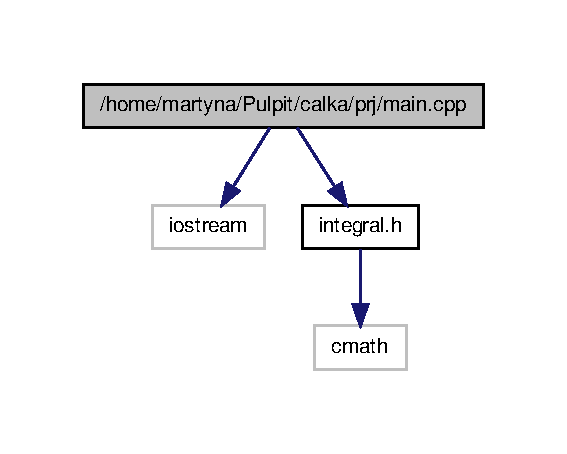
\includegraphics[width=272pt]{main_8cpp__incl}
\end{center}
\end{figure}
\subsection*{\-Funkcje}
\begin{DoxyCompactItemize}
\item 
double \hyperlink{main_8cpp_a80abd7257657e8a5b78f917731d87ba5}{\-F} (double x)
\item 
int \hyperlink{main_8cpp_ae66f6b31b5ad750f1fe042a706a4e3d4}{main} ()
\end{DoxyCompactItemize}


\subsection{\-Opis szczegółowy}
\-Plik zawiera glowna funkcje programu. 

\-Definicja w pliku \hyperlink{main_8cpp_source}{main.\-cpp}.



\subsection{\-Dokumentacja funkcji}
\hypertarget{main_8cpp_a80abd7257657e8a5b78f917731d87ba5}{\index{main.\-cpp@{main.\-cpp}!\-F@{\-F}}
\index{\-F@{\-F}!main.cpp@{main.\-cpp}}
\subsubsection[{\-F}]{\setlength{\rightskip}{0pt plus 5cm}double {\bf \-F} (
\begin{DoxyParamCaption}
\item[{double}]{x}
\end{DoxyParamCaption}
)}}\label{main_8cpp_a80abd7257657e8a5b78f917731d87ba5}


\-Definicja w linii 11 pliku main.\-cpp.



\-Oto graf wywoływań tej funkcji\-:\nopagebreak
\begin{figure}[H]
\begin{center}
\leavevmode
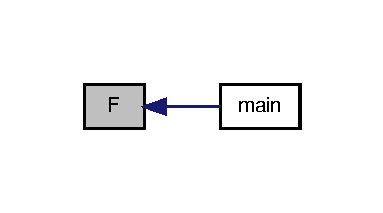
\includegraphics[width=184pt]{main_8cpp_a80abd7257657e8a5b78f917731d87ba5_icgraph}
\end{center}
\end{figure}


\hypertarget{main_8cpp_ae66f6b31b5ad750f1fe042a706a4e3d4}{\index{main.\-cpp@{main.\-cpp}!main@{main}}
\index{main@{main}!main.cpp@{main.\-cpp}}
\subsubsection[{main}]{\setlength{\rightskip}{0pt plus 5cm}int {\bf main} (
\begin{DoxyParamCaption}
{}
\end{DoxyParamCaption}
)}}\label{main_8cpp_ae66f6b31b5ad750f1fe042a706a4e3d4}


\-Definicja w linii 15 pliku main.\-cpp.



\-Oto graf wywołań dla tej funkcji\-:\nopagebreak
\begin{figure}[H]
\begin{center}
\leavevmode
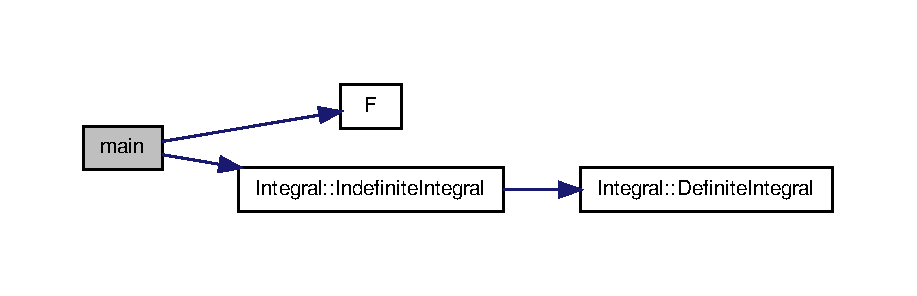
\includegraphics[width=350pt]{main_8cpp_ae66f6b31b5ad750f1fe042a706a4e3d4_cgraph}
\end{center}
\end{figure}



\printindex
\end{document}
